%!TEX program = xelatex
\documentclass[8pt, landscape, a4paper]{extarticle}

% --- 核心宏包 ---
\usepackage[UTF8, fontset=fandol]{ctex}
\usepackage[margin=0.8cm, top=1cm, bottom=1.3cm]{geometry}
\usepackage{multicol}
\usepackage{xcolor}
\usepackage{tcolorbox}
\usepackage{enumitem}
\usepackage{amsmath}
\usepackage{amssymb}
\usepackage{fontspec}
\usepackage{tikz}
\usetikzlibrary{arrows.meta, shapes.geometric, calc}

% --- 去掉页码 ---
\pagestyle{empty}

% --- 颜色定义 (红色主题) ---
\definecolor{headerblue}{RGB}{192, 57, 43}     % Pomegranate (深红)
\definecolor{navcolor}{RGB}{211, 84, 0}        % 导航橙
\definecolor{intuitioncolor}{RGB}{41, 128, 185}% 直觉蓝
\definecolor{accentcolor}{RGB}{142, 68, 173}   % 强调紫
\definecolor{section2}{RGB}{22, 160, 133}      % 绿色
\definecolor{dividergray}{RGB}{220, 220, 220}

% --- 全局设置 ---
\setlength{\parindent}{0pt}
\setlength{\columnsep}{0.4cm} 
\linespread{1.1} 

% --- 列表样式 ---
\setlist[itemize]{leftmargin=1.2em, nosep, itemsep=2pt, topsep=2pt, label=$\textcolor{headerblue}{\vcenter{\hbox{\tiny$\bullet$}}}$ }
\setlist[description]{leftmargin=0.2em, style=sameline, nosep, itemsep=2pt, font=\bfseries}

% --- Box 样式 ---
\newtcolorbox{mybox}[2][]{%
  colback=white,
  colframe=#2,
  coltitle=white,
  boxrule=1pt,             
  arc=2mm,                 
  left=4pt, right=4pt, top=3pt, bottom=3pt, 
  toptitle=3pt, bottomtitle=3pt, 
  fonttitle=\bfseries\sffamily\large,
  title={#1},
  after skip=5pt          
}

% --- 自定义命令 ---
\newcommand{\subt}[1]{{\vspace{2pt}\textbf{\large \textcolor{black}{#1}}}}

\newcommand{\boxdesc}[1]{%
    \textit{\small \textcolor{gray}{#1}}%
    \par\vspace{2pt}%
    {\color{dividergray}\hrule height 0.5pt}%
    \vspace{2pt}%
}

\newcommand{\sepline}{%
    \par \vspace{3pt}%
    {\color{dividergray}\hrule height 0.5pt}%
    \par \vspace{3pt}%
}

% 公式间距
\setlength{\abovedisplayskip}{3pt}
\setlength{\belowdisplayskip}{3pt}

\begin{document}

% --- 页眉 ---
\begin{center}
    {\Huge \textbf{\sffamily \textcolor{headerblue}{抽象代数 Abstract Algebra Cheat Sheet}}} \\
    \vspace{0.2cm}
    {\large \texttt{The Rules of Structure: From Groups to Cryptography}}
\end{center}

% --- 开始四栏布局 ---
\begin{multicols*}{4}

% === 第一栏 ===

\begin{mybox}[️ 场景导航 (Use Cases)]{navcolor}
    \boxdesc{遇到什么问题 $\to$ 用什么工具}
    \begin{itemize}[itemsep=2pt]
        \item \textbf{数据加密/签名} $\to$ 群论 / 椭圆曲线 (ECC)
        \item \textbf{数据校验/纠错} $\to$ 有限域 (Galois Field)
        \item \textbf{冗余编码 (RAID)} $\to$ 多项式环
        \item \textbf{对称性分析} $\to$ 置换群
        \item \textbf{类型系统设计} $\to$ 范畴论 / 同态
        \item \textbf{零知识证明} $\to$ 算术电路 / 多项式承诺
    \end{itemize}
\end{mybox}

\begin{mybox}[1. 群论 (Groups)]{headerblue}
    \boxdesc{对称性的数学描述}
    
    \subt{定义 $(G, \cdot)$}
    集合 $G$ 和运算 $\cdot$ 满足:
    \begin{itemize}
        \item \textbf{封闭性}: $a \cdot b \in G$。
        \item \textbf{结合律}: $(a \cdot b) \cdot c = a \cdot (b \cdot c)$。
        \item \textbf{单位元}: $\exists e, a \cdot e = a$。
        \item \textbf{逆元}: $\forall a, \exists a^{-1}, a \cdot a^{-1} = e$。
    \end{itemize}
    \sepline
    
    \subt{关键概念}
    \begin{itemize}
        \item \textbf{阿贝尔群}: 交换律成立 ($ab=ba$)。
        \item \textbf{循环群}: 由一个元素生成 ($g^k$)。
        \item \textbf{阶 (Order)}: 元素个数 $|G|$。
        \item \textbf{拉格朗日定理}: 子群的阶整除群的阶。
        \item \textbf{正规子群}: 左右陪集相等,商群构造的基础。
        \item \textbf{凯莱定理}: 任何群都同构于某个置换群。
    \end{itemize}
\end{mybox}

\begin{mybox}[2. 环与域 (Rings \& Fields)]{headerblue}
    \boxdesc{加法与乘法的游乐场}
    
    \subt{环 (Ring)}
    有加法和乘法 (如整数 $\mathbb{Z}$)。
    \textit{注意: 乘法不一定有逆元 (不能除)。}
    \textbf{整环}: 无零因子 ($ab=0 \implies a=0 \lor b=0$)。
    \sepline
    
    \subt{域 (Field)}
    加减乘除都完备 (如 $\mathbb{R}, \mathbb{C}, \mathbb{Q}$)。
    \begin{itemize}
        \item \textbf{有限域 (Galois Field)}: 元素个数有限。
        \item 记作 $GF(p^n)$ 或 $\mathbb{F}_{p^n}$。
        \item \textbf{计算机最爱}: $GF(2^8)$ (Byte)。
    \end{itemize}
\end{mybox}

\columnbreak

% === 第二栏 ===

\begin{mybox}[3. 同态与同构 (Morphisms)]{headerblue}
    \boxdesc{结构之间的映射}
    
    \subt{同态 (Homomorphism)}
    保持运算结构的映射 $\phi$:
    $$ \phi(a \cdot b) = \phi(a) \star \phi(b) $$
    \textit{直觉: 在 A 世界运算后再过去,等于先过去再在 B 世界运算。}
    \sepline
    
    \subt{同构 (Isomorphism)}
    双射同态。两个结构本质相同,只是名字不同。
    \textit{例: 对数函数是 $(\mathbb{R}^+, \times) \to (\mathbb{R}, +)$ 的同构。}
    \sepline
    
    \subt{核 (Kernel)}
    映射到单位元的元素集合。$\text{Ker}(\phi) = \{x | \phi(x) = e'\}$。
    \sepline
    
    \subt{第一同构定理}
    $G / \text{Ker}(\phi) \cong \text{Im}(\phi)$。
    \textit{意义: 压缩掉核,剩下的结构就是像。}
    \sepline
    
    \subt{自同构 (Automorphism)}
    到自身的同构。$\text{Aut}(G)$ 构成群。
    \textit{例: 复数共轭 $z \mapsto \bar{z}$。}
\end{mybox}

\begin{mybox}[4. 密码学应用 (Crypto)]{headerblue}
    \boxdesc{基于“难解问题”的安全}
    
    \subt{RSA 算法}
    基于\textbf{大数分解}困难。
    \begin{itemize}
        \item 公钥 $(n, e)$, 私钥 $d$。
        \item 加密 $c = m^e \pmod n$。
        \item 解密 $m = c^d \pmod n$。
        \item 原理: 欧拉定理 $m^{\phi(n)} \equiv 1 \pmod n$。
    \end{itemize}
    \sepline
    
    \subt{Diffie-Hellman 密钥交换}
    基于\textbf{离散对数}困难 ($g^x \pmod p$ 求 $x$)。
    \begin{itemize}
        \item Alice: $A = g^a$, Bob: $B = g^b$。
        \item 共享密钥: $S = B^a = (g^b)^a = g^{ab} = A^b$。
    \end{itemize}
    \sepline
    
    \subt{椭圆曲线 (ECC)}
    群运算定义在如下曲线的点集上:
    $$ y^2 \equiv x^3 + ax + b \pmod p $$
    \textit{优势: 相同安全强度下,密钥更短。}
    \sepline

    \subt{ElGamal 加密}
    基于离散对数,由 DH 扩展而来。
    \textit{特点: 引入随机数,同一明文对应不同密文。}
\end{mybox}

\columnbreak

% === 第三栏 ===

\begin{mybox}[5. 编码理论 (Coding Theory)]{headerblue}
    \boxdesc{对抗噪声与错误}
    
    \subt{汉明距离 (Hamming Dist)}
    两个码字不同位的个数。
    \textit{纠错能力: 若最小距离为 $d$,能纠正 $(d-1)/2$ 个错误。}
    \sepline
    
    \subt{CRC (循环冗余校验)}
    把数据看作多项式 $M(x)$,除以生成多项式 $G(x)$,余数即校验码。
    \textit{本质: 多项式环 $\mathbb{F}_2[x]$ 上的模运算。}
    \sepline
    
    \subt{里德-所罗门码 (Reed-Solomon)}
    \begin{itemize}
        \item 把数据点视为多项式系数。
        \item 过 $k$ 点可确定 $k-1$ 次多项式。
        \item 只要收到任意 $k$ 个分片,就能恢复原数据。
        \item \textbf{应用}: 二维码, RAID 6, 卫星通信。
    \end{itemize}
\end{mybox}

\begin{mybox}[6. 范畴论基础 (Category)]{headerblue}
    \boxdesc{数学的数学 (Meta-Math)}
    
    \subt{范畴 (Category)}
    对象 (Object) + 态射 (Morphism)。
    \sepline
    
    \subt{函子 (Functor)}
    范畴间的映射,保持结构。
    \texttt{List<T>} 就是一个 Functor (map)。
    \sepline
    
    \subt{单子 (Monad)}
    自函子范畴上的幺半群。
    \textit{程序员视角: 一种设计模式,用于处理副作用 (IO, Option, Future)。}
    $$ \text{bind}: M(a) \to (a \to M(b)) \to M(b) $$
\end{mybox}

\begin{mybox}[7. Python / SymPy 实战]{headerblue}
    \boxdesc{符号计算}
    \begin{itemize}
        \item \texttt{import sympy}
        \item \textbf{模逆}: \texttt{pow(a, -1, n)}
        \item \textbf{素数}: \texttt{sympy.isprime(n)}
        \item \textbf{有限域}: \texttt{GF(2**8)}
        \item \textbf{生成群}: \texttt{PermutationGroup(...)}
        \item \textbf{欧拉函数}: \texttt{sympy.totient(n)}
    \end{itemize}
\end{mybox}

\columnbreak

% === 第四栏 ===

\begin{mybox}[8. 高阶概念 (Advanced)]{headerblue}
    \boxdesc{通向现代数学}
    
    \subt{同调代数 (Homology)}
    用代数方法研究拓扑空间的“洞”。
    \textit{应用: 拓扑数据分析 (TDA)。}
    \sepline
    
    \subt{李群与李代数 (Lie Group)}
    既是群又是流形 (光滑连续)。
    \textit{应用: 机器人旋转控制 ($SO(3)$), 粒子物理。}
    \sepline
    
    \subt{格 (Lattice)}
    偏序集合,任意两元素有上确界和下确界。
    \textit{应用: 形式化验证, 密码分析。}
    \sepline
    
    \subt{表示论 (Representation)}
    把群元素映射为矩阵,用线性代数研究群。
\end{mybox}

\vspace*{\fill}

\begin{mybox}[ 核心直觉 (Intuition)]{intuitioncolor}
    \boxdesc{“结构决定性质。”}
    
    % TikZ 矢量图: 展示同态映射或循环群结构
    \begin{center}
    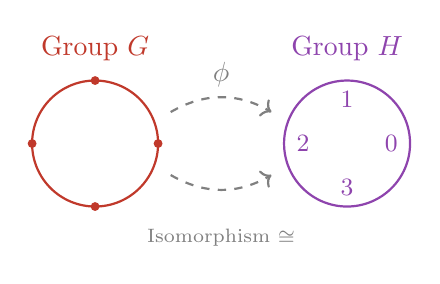
\begin{tikzpicture}[scale=0.8]
        % 左边的群 G (正方形对称群)
        \node[headerblue] at (-2, 1.5) {Group $G$};
        \draw[thick, headerblue] (-2,0) circle (1cm);
        \foreach \a in {0, 90, 180, 270}
            \fill[headerblue] (-2,0) ++(\a:1) circle (2pt);
        
        % 右边的群 H (整数模4)
        \node[accentcolor] at (2, 1.5) {Group $H$};
        \draw[thick, accentcolor] (2,0) circle (1cm);
        \foreach \a/\t in {0/0, 90/1, 180/2, 270/3}
            \node[accentcolor] at ($(2,0) + (\a:0.7)$) {\small \t};
            
        % 映射箭头
        \draw[->, thick, gray, dashed] (-0.8, 0.5) to[bend left] node[above] {$\phi$} (0.8, 0.5);
        \draw[->, thick, gray, dashed] (-0.8, -0.5) to[bend right] (0.8, -0.5);
        
        \node[gray, font=\scriptsize] at (0, -1.5) {Isomorphism $\cong$};
    \end{tikzpicture}
    \end{center}

    \hspace{1em}抽象代数让你忘掉数字的具体大小,只关注\textbf{运算规则}。
    \vspace{4pt}
    
    \subt{三大核心视角}
    \begin{itemize}[itemsep=4pt]
        \item \textbf{群即对称}: 
        研究一个物体怎么转动、翻转后保持不变。物理定律的守恒性 (诺瑟定理) 本质上就是群的对称性。
        
        \item \textbf{域即算术}: 
        如果你想在计算机里做完美的加减乘除 (没有浮点误差),你就需要有限域。它是现代编码和密码学的基石。
        
        \item \textbf{同态即翻译}: 
        把一个复杂系统映射到一个简单系统,如果结构保持不变,我们就可以在简单系统里解决问题,再翻译回去。
    \end{itemize}
    
    \vspace{6pt}
    \centering\textit{\footnotesize 所谓理解,就是发现不同事物背后的同一模式。}
\end{mybox}

\end{multicols*}

\end{document}
